\appendix
\chapter{Security Implementation}




\begin{lstlisting}[style=typescript,caption=Input Validation,label=apendix:input_val]
import {z} from "zod";

export const authorizationSchema = z.object({
    response_type: z.literal('code').optional() ,
    username: z.string(),
    password: z.string(),
    client_id: z.string(),
    redirect_uri: z.string().url().optional() ,
    scope: z.string().optional() ,
    state: z.string().optional() ,
    codeChallenge: z.string(),
    code_challenge_method: z.literal('S256').optional() ,
});

export const tokenRequestSchema = z.object({
    grant_type: z.literal('authorization_code'),
    authorizationCode: z.string(),
    redirect_uri: z.string().url().optional(),
    client_id: z.string(),
    codeVerifier: z.string()
});

\end{lstlisting}

\newpage
\begin{lstlisting}[style=typescript,caption=Code Challenge Validation,label=apendix:code_chal_val]
export const isCodeChallengeValid = (data: string): boolean => {
    const validLength = data.length >= 43 && data.length <= 128;
    // This code challenge is base64url encoded
    const validCharset = /^[A-Za-z0-9-._~]+$/.test(data);
    return validLength && validCharset;
}
\end{lstlisting}

\begin{lstlisting}[style=typescript,caption=Code Challenge Timing safe comparisons,label=apendix:timing_safe_comparions]
import crypto from 'crypto';

export const verifySHA = async (toVerify: string, expectedHash: string): Promise<boolean> => {
    const hash = await sha256(toVerify);
    // convert the hash to base64 url safe encoding without padding
    const base64Hash = Buffer.from(hash, 'hex').toString('base64').replace(/=+$/, '').replace(/\+/g, '-').replace(/\//g, '_');
    // prevent timing attacks by using crypto.timingSafeEqual
    return crypto.timingSafeEqual(Buffer.from(base64Hash), Buffer.from(expectedHash));
};
\end{lstlisting}

\newpage

\begin{lstlisting}[style=typescript,caption=Token Signature using Assymetric key with RS256 stored in Secrets Manager,label=apendix:token_signing]
import { SecretsManagerClient, GetSecretValueCommand } from '@aws-sdk/client-secrets-manager';
const client = new SecretsManagerClient({ region: 'us-east-1' });
export const getSecret = async (secretName: string): Promise<string> => {
    try {
        const command = new GetSecretValueCommand({ SecretId: secretName });
        const data = await client.send(command);
        if (data && data.SecretString) {
            return data.SecretString;
        } else {
            throw new Error('Secret binary data is not supported');
        }
    } catch (error) {
        console.error(`Error retrieving secret ${secretName}:`, error);
        throw error;
    }
};

// Load the private key from Secrets Manager
const privateKey = await getSecret('private_key');
// Generate JWT token
const token = jwt.sign(
    {
        userId: data.Items[0].id.S
    },
    privateKey, // Replace with your secret key
    {
        expiresIn: '1h',
        algorithm: 'RS256',
    }
);

\end{lstlisting}


\begin{lstlisting}[caption={Terraform For Least Privilidge}, label={apendix:least_privilidge}]
# IAM Policy for Lambda to log to CloudWatch
resource "aws_iam_policy" "private_key_read_policy" {
  name        = "private_key_read_policy"
  description = "IAM policy to allow Lambda to read private key from secret manager"

  policy = jsonencode({
    Version = "2012-10-17",
    Statement = [
      {
        Effect = "Allow",
        Action = [
          "secretsmanager:GetSecretValue"
        ],
        Resource = aws_secretsmanager_secret.private_key.arn
      }
    ]
  })
}

module "pkce_authorize_lambda" {
  source               = "./module/lambda"
  lambda_function_name = "authorizePKCE"
  source_dir           = "deployment/authorizePKCE"
  policies = [
    aws_iam_policy.lambda_dynamodb_policy.arn,
    aws_iam_policy.lambda_cloudwatch_policy.arn
  ]
}

module "pkce_token_lambda" {
  source               = "./module/lambda"
  lambda_function_name = "tokenPKCE"
  source_dir           = "deployment/tokenPKCE"
  policies = [
    aws_iam_policy.lambda_dynamodb_policy.arn,
    aws_iam_policy.lambda_cloudwatch_policy.arn,
    aws_iam_policy.private_key_read_policy.arn
  ]
}
\end{lstlisting}

\begin{lstlisting}[style=typescript,caption=Cross Tenant Data Leakage Integration Test ,label=apendix:cross_tenant_data_integ_test]
    import axios from 'axios';

// o6mwkkwazm - is the resapi id and this must be replaced with your own restapi-id from the output
const url = 'http://tenant1.local:4566/restapis/o4qbjcrrti/dev/_user_request_/authorize';
const headers = {
    'Content-Type': 'application/json',
};

describe('Integration testing POST /authorize', () => {
    test("test when tenant 1 and tenant 2 but when user from tenant 2 is tried to access from tenant-1 then access denied", async() => {
        const payload = {
            username: "user7@example.com",
            password: "test2",
            codeChallenge: "VkTJmESMq3DOD-fXIwqnD8ENlEOd2Prm3x8zO6u67aA",
            client_id: "tenant1-client-id-1"
        }

        try {
            await axios.post(url, payload, {headers, timeout: 30000});
        } catch (error) {
            console.log("Received response:", error);
            if (axios.isAxiosError(error) && error.response){
                expect(error.response.status).toBe(401);
            }
        }
    }, 50000)

    test("test when tenant 1 and tenant 2 but when client from tenant 2 is tried to access from tenant-1 host then access denied", async() => {
        const payload = {
            username: "user7@example.com",
            password: "test2",
            codeChallenge: "VkTJmESMq3DOD-fXIwqnD8ENlEOd2Prm3x8zO6u67aA",
            client_id: "tenant2-client-id-1"
        }

        try {
            await axios.post(url, payload, {headers, timeout: 30000});
        } catch (error) {
            console.log("Received response:", error);
            if (axios.isAxiosError(error) && error.response){
                expect(error.response.status).toBe(401);
            }
        }
    }, 50000)
});
\end{lstlisting}


\begin{lstlisting} [style=typescript,caption=Test Code Verifier and Code Challenge Input,label=apendix:rfc7636_test]
    it('should return 400 if code challenge is short', async () => {
        const mockEventShort: APIGatewayProxyEvent = {
            headers: { 'tenant-id': 'test-tenant' },
            body: JSON.stringify({ username: 'testuser', password: 'testpass', codeChallenge: generateRandomString(42), client_id: 'client1' }),
            // other properties can be added as needed
        } as any;
        const event = { ...mockEventShort};
        const response = await handler(event);
        expect(response.statusCode).toBe(400);
        expect(JSON.parse(response.body).message).toBe("Missing 'username', 'password', or 'codeChallenge' in request body");
    });

    it('should return 400 if code challenge is long', async () => {
        const mockEventShort: APIGatewayProxyEvent = {
            headers: { 'tenant-id': 'test-tenant' },
            body: JSON.stringify({ username: 'testuser', password: 'testpass', codeChallenge: generateRandomString(129), client_id: 'client1' }),
            // other properties can be added as needed
        } as any;
        const event = { ...mockEventShort};
        const response = await handler(event);
        expect(response.statusCode).toBe(400);
        expect(JSON.parse(response.body).message).toBe("Missing 'username', 'password', or 'codeChallenge' in request body");
    });
\end{lstlisting}
    
\begin{lstlisting}[style=typescript,caption=Timing test for Hash Comparision,label=apendix:timing_test]
import {QueryCommandOutput} from "@aws-sdk/client-dynamodb";
import {validateUserCredentials} from "../../src/utils/validateUserCredentials";
import * as argon2 from 'argon2';
import jstat from 'jstat';

const NUMBER_OF_ITERATIONS = 100;
const CORRECT_PASSWORD = "correct_pass";
describe('validateUserCredentials timing test', () => {
    const NON_MATCHING_PASSWORDS: number[] = [];
    const MATCHING_PASSWORDS: number[] = [];

    afterAll(() => {
        // eslint-disable-next-line security-node/detect-crlf
        console.log("p-Value", calculateChiSquare(NON_MATCHING_PASSWORDS, MATCHING_PASSWORDS))
    });

    it('running time test for incorrect passwords', async () => {
        const hash = await argon2.hash("correct_pass", {
            type: argon2.argon2id,
            memoryCost: 65536, // 64MB in KiB
            timeCost: 3,      // iterations
            parallelism: 4,   // parallel threads
            hashLength: 32    // output length in bytes
        });
        const userData: QueryCommandOutput = {
            Items: [{
                password: {
                    S: hash
                }
            }], $metadata: {}
        };

        for (let i = 0; i < NUMBER_OF_ITERATIONS; i++) {
            const incorrect_pass = generateRandomString(125)
            const startMatching = performance.now();
            const result = await validateUserCredentials('username', incorrect_pass, userData);
            const endMatching = performance.now();
            NON_MATCHING_PASSWORDS.push(endMatching - startMatching);
            expect(result).toBe(false);
        }
        console.table(NON_MATCHING_PASSWORDS);
    });

    it('running time test for correct passwords', async () => {
        const hash = await argon2.hash(CORRECT_PASSWORD, {
            type: argon2.argon2id,
            memoryCost: 65536, // 64MB in KiB
            timeCost: 3,      // iterations
            parallelism: 4,   // parallel threads
            hashLength: 32    // output length in bytes
        });
        const userData: QueryCommandOutput = {
            Items: [{
                password: {
                    S: hash
                }
            }], $metadata: {}
        };

        for (let i = 0; i < NUMBER_OF_ITERATIONS; i++) {
            const startMatching = performance.now();
            const result = await validateUserCredentials('username', CORRECT_PASSWORD, userData);
            const endMatching = performance.now();
            MATCHING_PASSWORDS.push(endMatching - startMatching);
            expect(result).toBe(true);
        }
        console.table(MATCHING_PASSWORDS);
    });

});

const generateRandomString = (length: number): string => {
    const characters = 'ABCDEFGHIJKLMNOPQRSTUVWXYZabcdefghijklmnopqrstuvwxyz0123456789';
    let result = '';
    const charactersLength = characters.length;

    for (let i = 0; i < length; i++) {
        result += characters.charAt(Math.floor(Math.random() * charactersLength));
    }

    return result;
}


const calculateChiSquare = (sample1: number[], sample2: number[]) => {
    const degreesOfFreedom = sample1.length - 1;
    const chiSquared = sample1.reduce((sum, obs, i) => {
        const exp = sample2[i];
        return sum + Math.pow(obs - exp, 2) / exp;
    }, 0);
    const pValue = 1 - jstat.chisquare.cdf(chiSquared, degreesOfFreedom);
    return {chiSquared, pValue, degreesOfFreedom};
}

\end{lstlisting}


\begin{lstlisting}[style=typescript,caption=Fuzz Test,label=apendix:fuzz_test]
    test('should handle fuzzed payloads for codeChallenge', async () => {
        for (let i = 0; i < 10; i++) {
            const username = fc.sample(fc.string(), 1)[0];
            const password = fc.sample(fc.string(), 1)[0];
            const codeChallenge = fc.sample(fc.string(), 1)[0];
            console.log(`Fuzzing iteration ${i} with username: ${username}, password: ${password}, codeChallenge: ${codeChallenge}`);
            await fc.assert(
                fc.asyncProperty(
                    fc.record({
                        username: fc.constant(username),
                        password: fc.constant(password),
                        codeChallenge: fc.constant(codeChallenge),
                        client_id: fc.constant("tenant1-client-id-1"),
                    }),
                    async (payload) => {
                        console.log("Sending request with payload:", payload);
                        try {
                            const response = await axios.post(url, payload, {headers, timeout: 30000});
                            console.log("Received response:", response.status);
                            expect(response.status).toBe(200);
                        } catch (error) {
                            console.log("Error occurred:", error);
                            // Handle expected errors
                            if (axios.isAxiosError(error) && error.response) {
                                console.log("Axios error response:", error.response);
                                if (error.response.status === 401) {
                                    console.log("Received 401 Unauthorized");
                                    expect(error.response.status).toBe(401);
                                } else {
                                    expect(error.response.status).toBeGreaterThanOrEqual(400);
                                    expect(error.response.status).toBeLessThan(500);
                                }
                            } else {
                                throw error;
                            }
                        }
                    }
                )
            );
        }
    }, 300000); // Increase timeout to 5 Minutes
\end{lstlisting}
\begin{figure}[h!]
\label{fig:argon2id_hash}
\centering
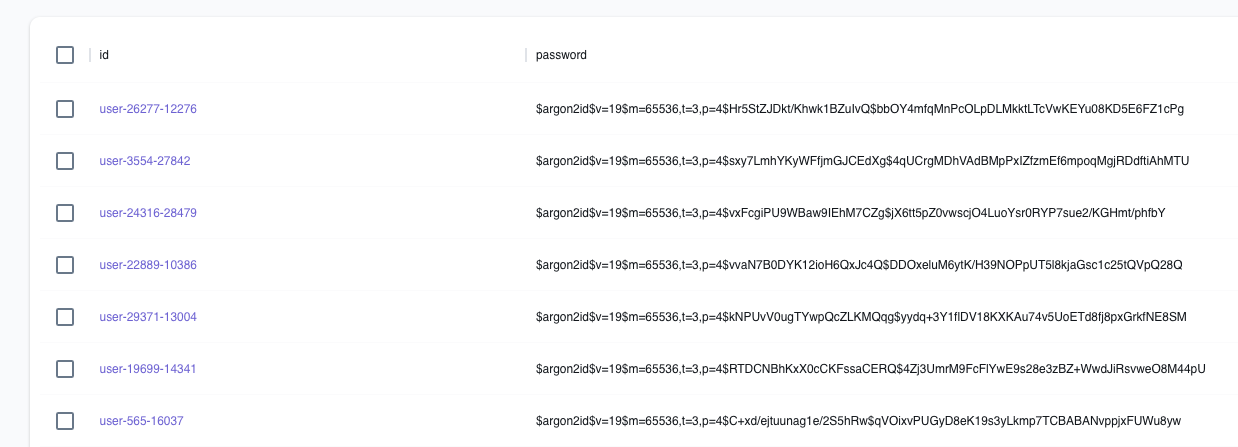
\includegraphics[width=\textwidth, height=200px]{pics/argon2id.png}
\caption{User Passwords hashed with Argon2id}
\end{figure}

\begin{figure}[!htbp]
    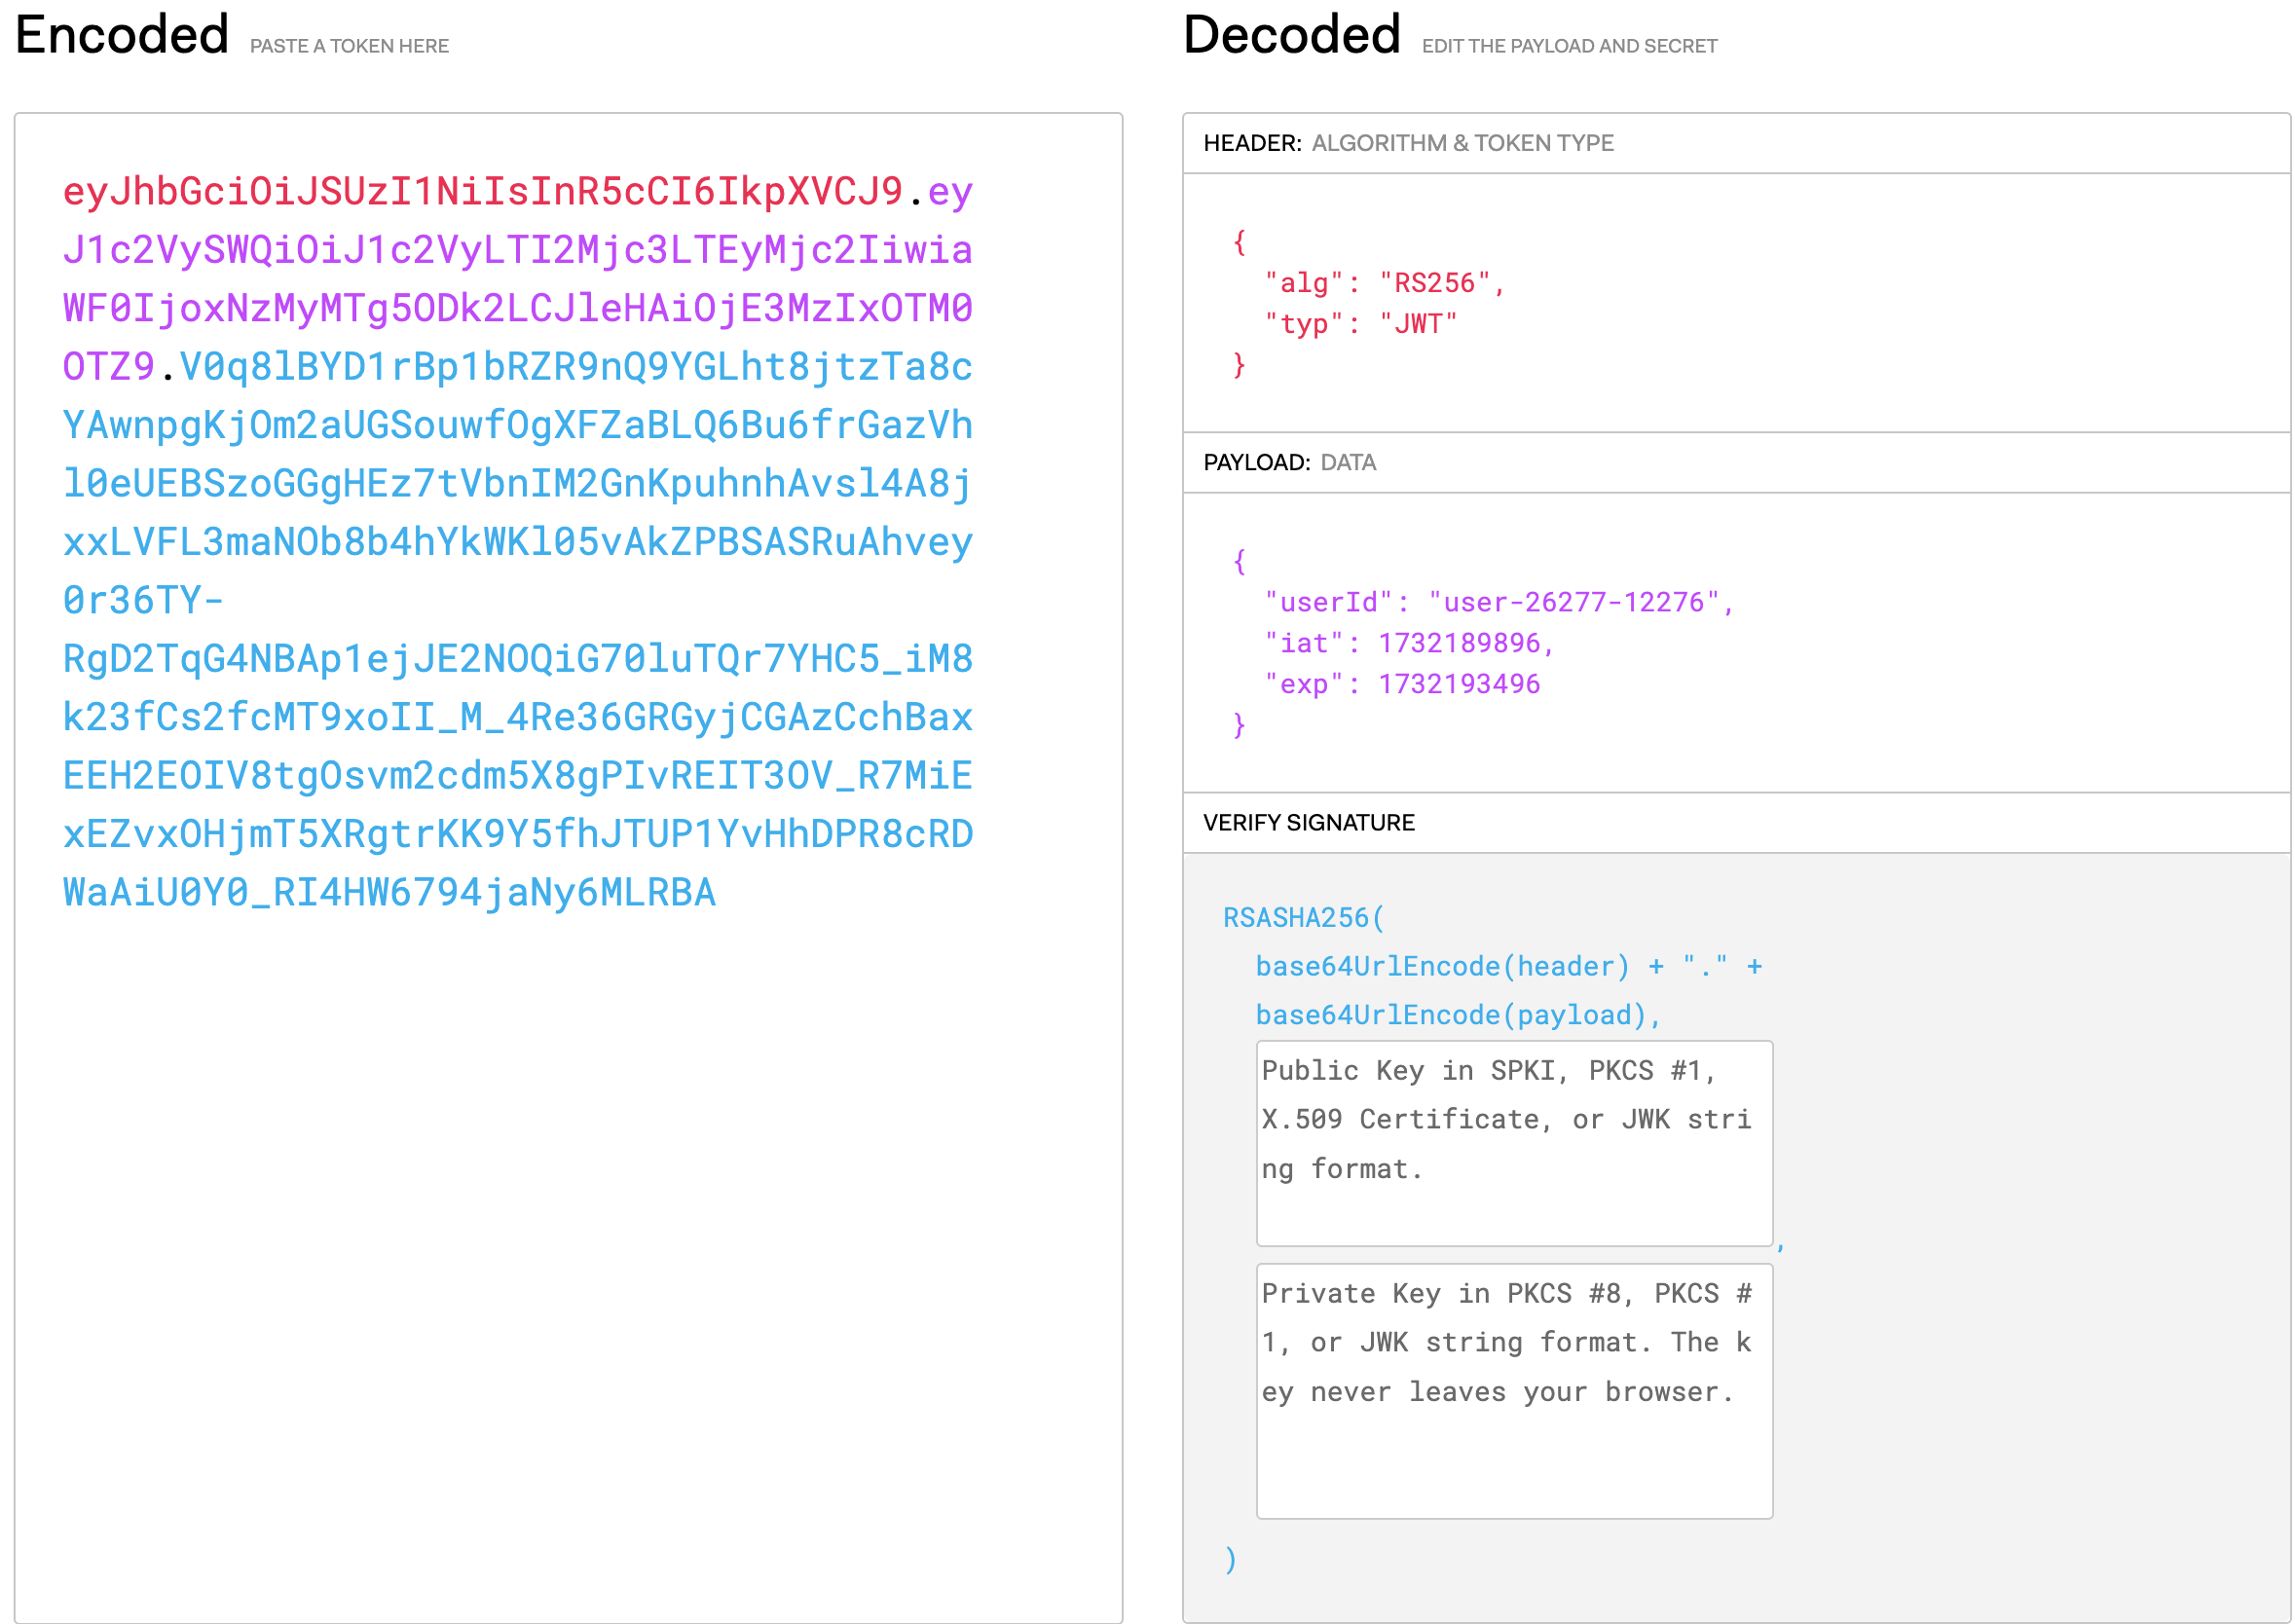
\includegraphics[width=\textwidth]{pics/token_signed.png}
    \caption{Signed Token with a symmetric key using RS256 for tamper protection}
    \label{fig:token_tenant_1_token_signed}
\end{figure}